\documentclass{beamer}
% imprimir
% \documentclass[handout]{beamer} 
% \usepackage{pgfpages}
% \pgfpagesuselayout{4 on 1}[a4paper,landscape,border shrink=5mm]

\mode<presentation> {
  \usetheme{Warsaw}
  \setbeamercovered{transparent}
}

\usebackgroundtemplate{
\includegraphics[width=\paperwidth]{format/libresoft-bg.png}}
\usepackage[spanish]{babel}
\usepackage[utf8]{inputenc}
\usepackage{graphics}
\usepackage{hyperref}
\usepackage{amssymb} % Simbolos matematicos

%\definecolor{libresoftgreen}{RGB}{162,190,43}
%\definecolor{libresoftblue}{RGB}{0,98,143}

%\setbeamercolor{titlelike}{bg=libresoftgreen}

%% Metadatos del PDF.
\hypersetup{  
  pdftitle={StaaS: el almacenamiento como servicio},
  pdfauthor={Miguel Vidal},
  pdfcreator={GSyC/Libresoft},
  pdfproducer=PDFLaTeX,
  pdfsubject={Curso Arquitectura Servidores},
}
%%


\defbeamertemplate*{footline}{shadow theme}
{%
  \leavevmode%
  \hbox{\begin{beamercolorbox}[wd=.5\paperwidth,ht=2.5ex,dp=1.125ex,leftskip=.3cm plus1fil,rightskip=.3cm]{author in head/foot}%
    \usebeamerfont{author in head/foot}\insertframenumber\,/\,\inserttotalframenumber\hfill
\includegraphics[scale=0.40]{format/cc-by-80x15.png} \hspace{0.1cm}\insertshortauthor 
% \usebeamerfont{author in head/foot} 
\includegraphics[width=0.7cm]{format/cc-by.png} \hfill\insertshortauthor
  \end{beamercolorbox}%
  \begin{beamercolorbox}[wd=.5\paperwidth,ht=2.5ex,dp=1.125ex,leftskip=.3cm,rightskip=.3cm plus1fil]{title in head/foot}%
    \usebeamerfont{title in head/foot}\insertshorttitle%
  \end{beamercolorbox}}%
  \vskip0pt%
}

\begin{document}

\title{StaaS: el almacenamiento como servicio (I)}
\subtitle{Curso Arquitectura de Servidores}
\institute{\{mvidal,jfcastro\}@libresoft.es} 
\author{Miguel Vidal, José Castro}
%\date{\today}
\date{6 de mayo de 2011}

\frame{
\maketitle
\begin{center}

\includegraphics[width=6cm]{format/gsyc-urjc}
\end{center}
}

%% License slide
\begin{frame}
  \vspace{2cm}
  \begin{flushright}
    {\footnotesize \copyright{} 2011 Miguel Vidal, Jose Castro.} \\
%    \vspace{0.25cm}
    \medskip
    {\scriptsize Esta presentación se distribuye bajo \\ licencia Creative Commons Reconocimiento 3.0 España}
%    \vspace{0.10cm}
  \end{flushright}
  \begin{center}
    \href{http://creativecommons.org/licenses/by/3.0/es}{
\includegraphics[width=2cm]{format/cc-by.png}} \\
    {\tiny \url{http://creativecommons.org/licenses/by/3.0/es}}
  \end{center}
\end{frame}%%


\normalsize

%Agenda
% \section*{Agenda}
\begin{frame}{Agenda}
\tableofcontents
\end{frame}


% Inicio de la presentacion

\begin{frame}
  \frametitle{Motivación}

Por qué estudiar las tecnologías de almacenamiento:

  \begin{itemize}
    \item Es una de las tecnologías básicas que se combina con clusters, virtualización y cloud computing. 
    \item Rendimiento y escalabilidad, replicación, migración no disruptiva de datos...
    \item Virtualización del almacenamiento.
    \item Reducción de los requerimientos de espacio y ahorro en costes de energía. 
  \end{itemize}
\end{frame}


\section{Sistemas de ficheros}

\begin{frame}
  \begin{center}
    \Huge{Sistemas de ficheros}
  \end{center}
\end{frame}


\begin{frame}
  \frametitle{¿Qué es un sistema de ficheros?}
  \begin{enumerate}
    \item Permite al SO almacenar, organizar, manipular y recuperar datos.
    \item Es usado en toda clase de dispositivos de almacenamiento (discos duros, cdroms, etc.).
    \item *BSD (UFS/FFS), Familia Solaris (ZFS, UFS)
    \item Linux Second Extended Filesystem (ext2, ext3 o ext4): similar e inspirado por ufs/ffs.
    \item Sistema de archivos de red: NFS, SMB (CIFS)
    \item Sistemas de ficheros distribuidos: GFS, OCFS2
  \end{enumerate}

\small{\url{http://en.wikipedia.org/wiki/Comparison_of_file_systems}}

\end{frame}

\begin{frame}
  \frametitle{El sistema de ficheros}

¿Qué podemos encontrarnos en un ``sistema de ficheros''?

\pause

\begin{itemize}
\item Procesos

\pause

\item Puertos serie

\pause

\item Estructuras de datos del y parámetros de ajuste

\pause

\item Canales de comunicación entre procesos 

\pause

\item Ficheros


\end{itemize}

\pause

\begin{center}
\alert{Enfoque Unix: todo es un fichero}
\end{center}

\end{frame}

\begin{frame}
  \frametitle{El sistema de ficheros de Unix}

En abstracto, el sistema de ficheros de Unix comprende cuatro componentes principales:

  \begin{itemize}
    \item Un \alert{espacio de nombres}: un modo de nombrar las cosas y organizarlas en una jerarquía.
    \item Una \alert{API}: un conjunto de llamadas al sistema para navegar y manipular objetos.
    \item Un \alert{modelo de seguridad}: un esquema para proteger, olcutar y compartir cosas.
    \item Una \alert{implementación}: software que enlaza el modelo lógico con el hardware real.
  \end{itemize}
\end{frame}

\begin{frame}
  \frametitle{La organización del árbol de ficheros}

Estructura estándar de directorios:

  \begin{itemize}

\small
    \item \alert{\texttt{/bin}} Comandos necesarios para una mínima operabilidad del sistema 
    \item \alert{\texttt{/sbin}} Comandos para el arranque, reparación y recuperación del sistema
    \item \alert{\texttt{/boot}} Kernel y ficheros necesarios para cargar el kernel 
    \item \alert{\texttt{/lib}} Librerías y partes del compilador C
    \item \alert{\texttt{/etc}} Archivos de configuración y de inicio 
    \item \alert{\texttt{/dev}} Entradas de dispositivo para discos, impresoras, pseudo-terminales, etc.
    \item \alert{\texttt{/proc}} Información sobre procesos ejecutándose
    \item \alert{\texttt{/home}} Directorios personales de usuarios
    \item \alert{\texttt{/var}} Datos variables 
    \item \alert{\texttt{/tmp}} Ficheros temporales que desaparecen entre \textit{reboots}.
    \item \alert{\texttt{/root}} Directorio personal del superusuario 

  \end{itemize}

\normalsize

\end{frame}

\begin{frame}
  \frametitle{El sistema de ficheros}

Órdenes relativas a sistemas de ficheros Unix:

  \begin{itemize}
    \item \alert{\texttt{chmod}} El comando \texttt{chmod} cambia los permisos de un fichero.
    \item \alert{\texttt{chown}} El comando \texttt{chown} cambia el propietario y el grupo de un fichero.
    \item \alert{\texttt{umask}} Asigna los permisos por defecto.
  \end{itemize}



\begin{block}{Atributos de un fichero:}
\small
  \texttt{\# ls -l /bin/gzip} \\ 
  \texttt{-rwxr-xr-x 1 root root 57388 2010-01-19 22:45 /bin/gzip}
\end{block}

\normalsize
\end{frame}


\begin{frame}
  \frametitle{Journaling}
  \begin{itemize}
    \item Un sistema de ficheros que hace seguimiento de los cambios en un \textit{journal} antes de escribirlos en el sistema de ficheros.
    \item Incrementa la fiabilidad: puede mantener la consistencia del sistema de ficheros incluso ante incidencias inesperadas como cortes de energía, cuelgues o reinicios no previstos.
    \item Puede haber un gran impacto en el rendimiento (los datos se escriben dos veces): solo metadatos es un compromiso entre fiabilidad y rendimiento.
    \item Es una modificación conceptualmente simple que incrementa notablemente la fiabilidad: ext3, reiserfs, jfs, xfs, ext4, ntfs... 
  \end{itemize}
\end{frame}


\begin{frame}
  \frametitle{ext3fs}
  \begin{itemize}
    \item El sistema de ficheros principal de Linux.
    \item El código para ext2 fue escrito específicamente para Linux, adoptando muchos conceptos de Berkeley FFS/UFS (Unix BSD).
    \item Es una extensión a ext2fs que añade capacidad de \textit{journaling}.
    \item Las extensiones ext3fs se implementaron sin cambiar la estructura de ext2fs: puede montarse un sistema ext3fs como ext2fs (simplemente el \textit{journaling} quedaría desactivado).
  \end{itemize}
\end{frame}


\begin{frame}
  \frametitle{XFS y JFS}
  \begin{itemize}
    \item XFS (SGI) y JFS (IBM): mayores competidores de ext3 en Linux.
    \item Soportados nativamente por el kernel Linux y las distribuciones basadas en él.
    \item Alto rendimiento con journaling.
    \item XFS tiene mayor fragmentación y gestión extendida.
    \item El rendimiento general es similar a ext3fs (lo que ha motivado su escasa implantación).
  \end{itemize}
\end{frame}


%%%%%%%%%%%%%%%%%%%%%%%%%%%%%%%%%%%%%%%%%%%%%%%%%%%%%%%%%%%%%%%%%%%%%

\section{LVM}

\begin{frame}
  \begin{center}
    \Huge{Volúmenes Lógicos (LVM)}
  \end{center}
\end{frame}

\begin{frame}
  \frametitle{Antes de los volúmenes lógicos}
Al principio, cada sistema de ficheros manejaba un único disco:

\begin{figure}[h]
\begin{center}
  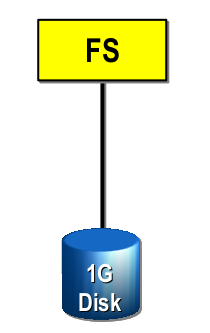
\includegraphics[width=3cm]{figs/singledisk.png}
  \caption{{\footnotesize No era muy grande.}}
\end{center}
\end{figure}

\end{frame}


\begin{frame}
  \frametitle{Por qué existen volúmenes lógicos}
Los usuarios precisaban más espacio, ancho de banda, fiabilidad y flexibilidad:

\begin{figure}[h]
\begin{center}
  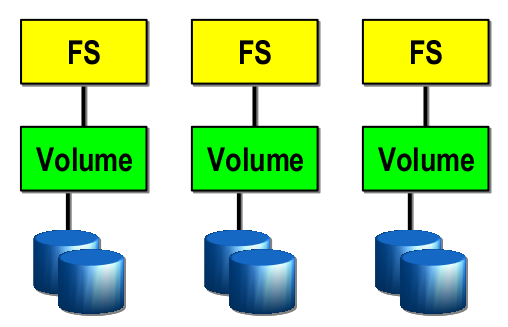
\includegraphics[width=6cm]{figs/volumes.png}
  \caption{{\footnotesize Fácil: inserta un ``volumen'' para juntar discos.}}
\end{center}
\end{figure}

\end{frame}



\begin{frame}
  \frametitle{Gestión de Volúmenes Lógicos (LVM)}
  \begin{itemize}
    \item Más flexible que los esquemas de particionado convencionales. 
    \item LVM permite que el espacio sea dinámicamente asignado desde una partición grande a las particiones que van necesitándose.
    \item Permite concatenar, dividir, juntar o cualquier otra combinación entre particiones en una partición virtual mayor, que los sysadmins pueden cambiar el tamaño o mover.
    \item Idealmente sin interrupción del sistema.
    \item LVM ayuda a los sysadmins a asignar el espacio disponible en disco entre particiones.
    \item LVM es una de las muchas formas de virtualización del almacenamiento. 
  \end{itemize}
\end{frame}

\begin{frame}
  \frametitle{Ejemplo de LVM en Linux}
\begin{figure}[h]
\begin{center}
  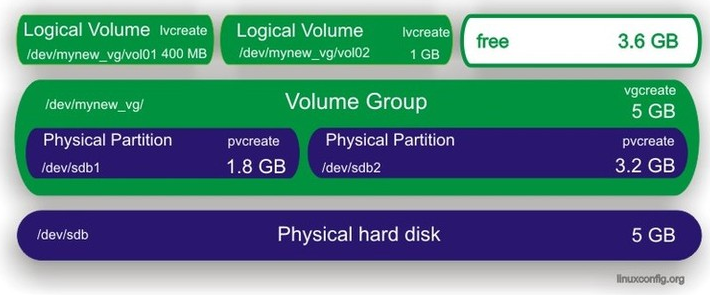
\includegraphics[width=11cm]{figs/lvm.png}
%  \caption{{\footnotesize Easy: insert a ``volume'' to cobble disks together.}}
\end{center}
\end{figure}
\end{frame}

\begin{frame}
  \frametitle{Ejemplo de LVM en Linux}

\begin{block}{Creación de volúmenes físicos}
  \texttt{\# pvcreate /dev/sdb1} \\
  \texttt{\# pvcreate /dev/sdb2}
\end{block}

\begin{block}{Creación del Virtual Group}
  \texttt{\# vgcreate mynew\_vg /dev/sdb1 /dev/sdb2 }
\end{block}

\begin{block}{Añadir nuevos volúmenes físicos a un grupo virtual}
  \texttt{\# vgextend mynew\_vg /dev/sdb3 } 
\end{block}

\end{frame}


\begin{frame}
  \frametitle{Ejemplo de LVM}

\begin{block}{Creación de Volúmenes Lógicos}
  \texttt{\# lvcreate -L 400 -n vol01 mynew\_vg } \\
  \texttt{\# lvcreate -L 1000 -n vol02 mynew\_vg }
\end{block}

\begin{block}{Mostrar Grupos y Volúmenes Lógicos}
  \texttt{\# vgdisplay } \\
  \texttt{\# lvdisplay }
\end{block}

\begin{block}{Creación de un sistema de ficheros en volúmenes lógicos}
  \texttt{\# mkfs.ext3 /dev/mynew\_vg/vol01} \\
  \texttt{\# mount /dev/mynew\_vg/vol01 /home/foobar}
\end{block}
\end{frame}

\begin{frame}
  \frametitle{Linux ext3 vs. ext4}
\begin{figure}[h]
\begin{center}
  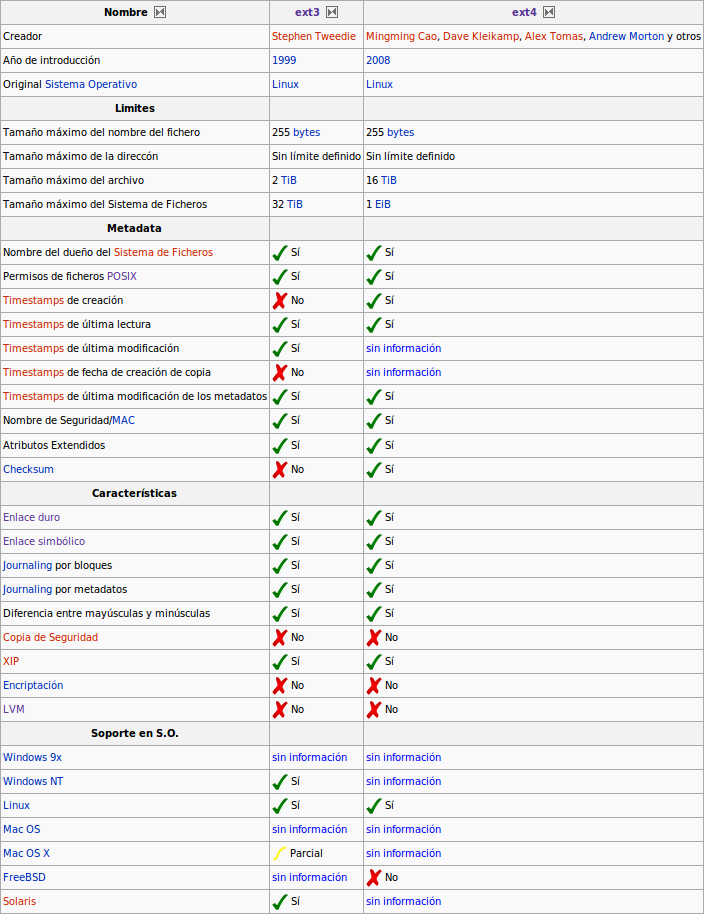
\includegraphics[width=10.5cm]{figs/Tabla_ext3_ext4.png}
\end{center}
\end{figure}
\end{frame}

\begin{frame}
  \frametitle{B-tree file system (btrfs)}
  \begin{itemize}
    \item Se propone reeemplazar ext3 y trasladar muchas de las funcionalidades de ZFS al mundo Linux (copy-on-write, snapshots, optimizado para SSD, etc.).
    \item Incorporado al kernel Linux 2.6.29 en enero 2009.
    \item  No apto para producción. Futuro incierto (es de Oracle, también dueña de ZFS)
    \item Pero se puede experimentar con él instalando \texttt{btrfs-tools} y \texttt{btrfsptogs} en Ubuntu u OpenSUSE. 
  \end{itemize}

\end{frame}



\section{RAID}

\begin{frame}
  \begin{center}
    \Huge{RAID}
  \end{center}
\end{frame}

\begin{frame}
  \frametitle{RAID: Redundant Array of Independent Disks}
  \begin{itemize}
    \item Es un sistema que utiliza varios discos duros para distribuir o replicar datos a través de los discos.
    \item Evita pérdida de datos.
    \item Minimiza los tiempos de caída asociados a fallos de hardware (a menudo los reduce a cero).
    \item También puede incrementar el rendimiento.
    \item Se puede implementar en el hardware o vía software.
  \end{itemize}
\end{frame}

\begin{frame}
  \frametitle{Redundant Array of Independent Disks}

RAID puede hacer dos cosas básicas:

  \begin{enumerate}
    \item Puede mejorar el rendimiento dividiendo (\alert{stripping}) los datos a través de varios discos, que trabajan simultáneamente con un flujo único de datos.
    \item Puede duplicar (\alert{mirror}) datos a través de varios discos, reduciendo el riesgo asociado al fallo de un disco.
  \end{enumerate}
\end{frame}


\begin{frame}
  \frametitle{Niveles estándar de RAID}

  \begin{itemize}
    \item \alert{RAID 0}: (\alert{stripping}) discos divididos sin paridad ni espejo
    \item \alert{RAID 1} (\alert{mirroring} o duplicación) es el primer nivel que ofrece redundancia.
    \item \alert{RAID 4} divide el volumen con paridad dedicada. Compite (y pierde en consistencia) con RAID 5.
    \item \alert{RAID 5} Volumen dividido (\textit{stripped}) con paridad distribuida. RAID 5 requiere al menos 3 discos.
    \item \alert{RAID 10} RAID 1+0 (o 10) es un volumen de datos espejado (RAID 1) que a su vez es dividido (RAID 0). RAID 10 requiere al menos 4 discos.
  \end{itemize}
\end{frame}

\begin{frame}
  \frametitle{RAID 0}

  \begin{itemize}
    \item \alert{RAID 0} (discos divididos sin paridad ni \alert{mirroring}): usa dos o más discos de igual tamaño para reducir los tiempos de acceso y escritura. Se emplea exclusivamente para mejorar rendimiento.
    \item Tolerancia a fallos: 0 discos
  \end{itemize}

\begin{figure}[h]
\begin{center}
  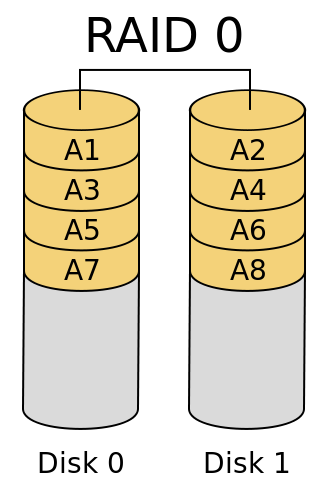
\includegraphics[width=2.5cm]{figs/RAID_0.png}
%  \caption  RAID level 0.
\end{center}
\end{figure}

\end{frame}

\begin{frame}
  \frametitle{RAID-1}

  \begin{itemize}
    \item Volumen duplicado (``espejado'') sin paridad ni stripping: ofrece redundancia. Los datos son duplicados en dos o más discos de forma simultánea.
    \item Tolerancia a fallos: n-1 discos
  \end{itemize}

\begin{figure}[h]
\begin{center}
  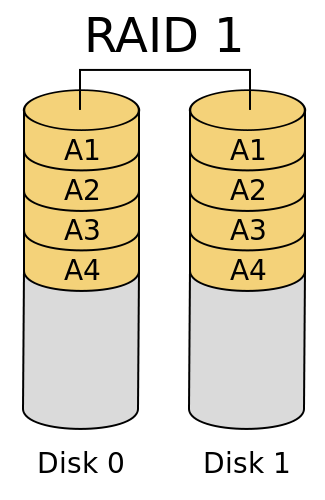
\includegraphics[width=2.5cm]{figs/RAID_1.png}
%  \caption  RAID level 1.
\end{center}
\end{figure}

\end{frame}

\begin{frame}
  \frametitle{RAID-4}

  \begin{itemize}
    \item Discos divididos con un disco dedicado a información de paridad. Por ello incurre en tiempos de espera cuando escribe la paridad, lo que hace que pierda con RAI-5, su competidor. Excepto que tengas una buena razón, descártalo en favor de RAID-5.
    \item Tolerancia a fallos: 1 discos
    \item RAID 5 requires at least 3 disk drives.
  \end{itemize}

\begin{figure}[h]
\begin{center}
  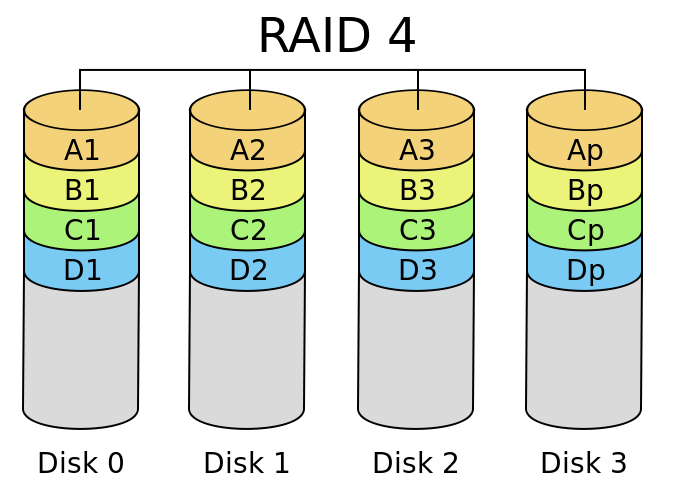
\includegraphics[width=3.5cm]{figs/RAID_4.png}
%  \caption  RAID level 4.
\end{center}
\end{figure}

\end{frame}


\begin{frame}
  \frametitle{RAID-5}

  \begin{itemize}
    \item Volumen dividido con paridad distribuida: es el nivel estándar más completo de RAID. Dividiendo datos e información de paridad, crea una arquitectura redundante que al mismo tiempo mejora los tiempos de lectura/escritura.
    \item Tolerancia a fallos: 1 disco.
    \item RAID 5 requiere al menos 3 discos.
  \end{itemize}

\begin{figure}[h]
\begin{center}
  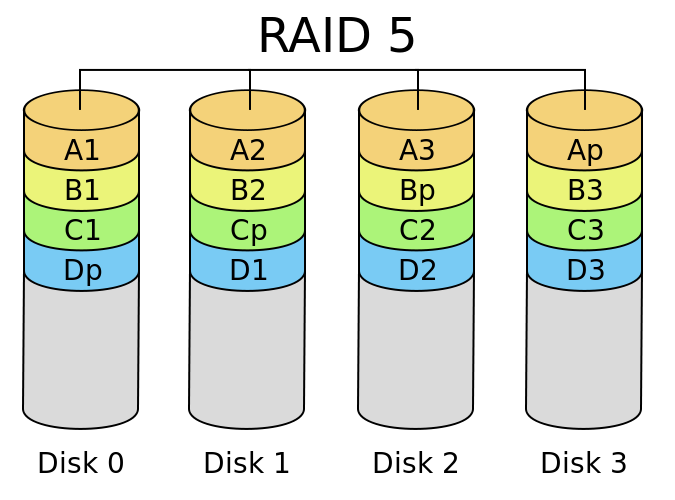
\includegraphics[width=4cm]{figs/RAID_5.png}
%  \caption  RAID level 5.
\end{center}
\end{figure}

\end{frame}


\section{ZFS}

\begin{frame}
  \begin{center}
    \Huge{ZFS}
  \end{center}
\end{frame}

\begin{frame}
  \frametitle{Un vistazo a ZFS}
  \begin{itemize}
    \item ZFS es un potente, escalable (128bit) y moderno sub-sistema de almacenamiento.
    \item Fiable, administración sencilla, integridad de datos y servicios integrados.
    \item ZFS combina los roles tradicionales de Volume Manager (RAID) y Sistema de Ficheros.
    \item La idea es que el disco debería ser algo similar a los módulos DIMM de RAM, conectar y usar.
    \item ZFS se lleva muy bien con SSD, y sabe cómo usarlo.
    
  \end{itemize}
\end{frame}



\begin{frame}
  \frametitle{ZFS: características únicas (1)}
  \begin{itemize}
    \item \textit{Pool} de almacenamiento: elimina por completo el viejo concepto de volumen lógico como capa aparte.
    \item ZFS es Copy-on-Write transaccional: si múltiples procesos piden recursos iguales, se les devuelven punteros al mismo recurso. 
    \item Siempre consistente (no necesidad de fsck)
    \item Integridad de datos: detecta y corrige silenciosamente corrupción de datos.
    \item Inmensa escalabilidad
  \end{itemize}

\end{frame}


\begin{frame}
  \frametitle{ZFS: características únicas (y 2)}
  \begin{itemize}
    \item Características avanzadas: snapshots, clones, rollbacks, deduplication, compresión, replicación, cifrado, compartición nativa vía nfs, cifs o iscsi...
    \item  Administración simple: \texttt{zfs} y \texttt{zpool}.
    \item Estado del arte, marca el camino a los futuros FS (como btrfs)
    \item Limitaciones: 
  \begin{itemize}
    \item ZFS no es un FS de tipo cluster ni un sistema distribuido o paralelo.
    \item Muy exigente en recursos.
  \end{itemize}
  \end{itemize}

En el proceso de escritura (I/O), un bloque puede ser comprimido, cifrado, realizada la suma de comprobación y a continuación deduplicado, en ese orden.

\end{frame}

%%%%%%%%%%%%%
\begin{frame}
  \frametitle{ZFS: pools de almacenamiento}

  \begin{center}
    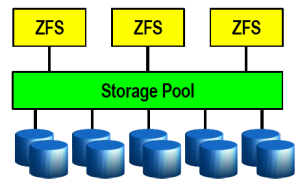
\includegraphics[height=2.5cm]{figs/zfs_storage_pool.png}
  \end{center}
  \begin{itemize}
    \item Los sistemas de ficheros se crean sobre pools de almacenamiento virtual llamados {\it zpools}.
    \item Un zpool se construye a partir de dispositivos virtuales ({\it vdevs}) desde dispositivos de bloques: ficheros, particiones de disco duro o discos enteros.
  \end{itemize}
\end{frame}


%%%%%%%%%%%%%
\begin{frame}
  \frametitle{Modo transaccional COW en ZFS}

  \begin{center}
    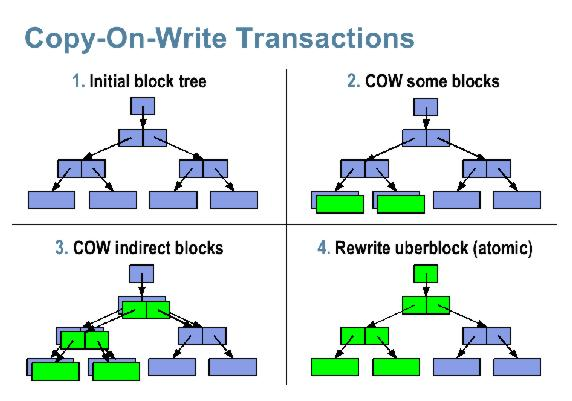
\includegraphics[height=2.5in]{figs/cow.jpg}
  \end{center}
\end{frame}



\begin{frame}
  \frametitle{Modelo Volumen/FS vs. Pool de almacenamiento}

Volúmenes tradicionales:

  \begin{itemize}
    \item Abstracción: disco virtual 
    \item Partición/volumen para cada FS      
    \item Crece o se reduce manualmente
    \item Cada FS tiene ancho de banda limitado
    \item El almacenamiento se fragmenta 
  \end{itemize}

\begin{figure}[h]
\begin{center}
  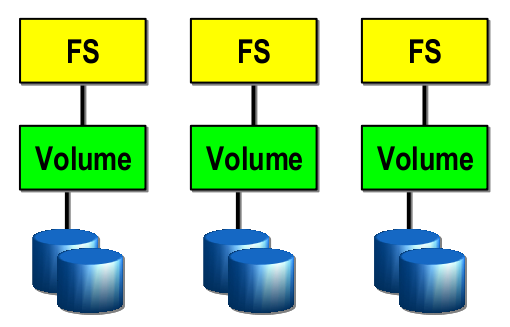
\includegraphics[width=5cm]{figs/volumes2.png}
\end{center}
\end{figure}

\end{frame}


\begin{frame}
  \frametitle{Modelo Volumen/FS vs. Pool de almacenamiento}

Almacenamiento con ZFS pools:

  \begin{itemize}
    \item Abstracción: malloc/free
    \item No hay particiones que manejar
    \item Crece o se reduce automáticamente
    \item Todo el ancho de banda está siempre disponible 
    \item Todo el almacenamiento en el pool es compartido 
  \end{itemize}
\begin{figure}[h]
\begin{center}
  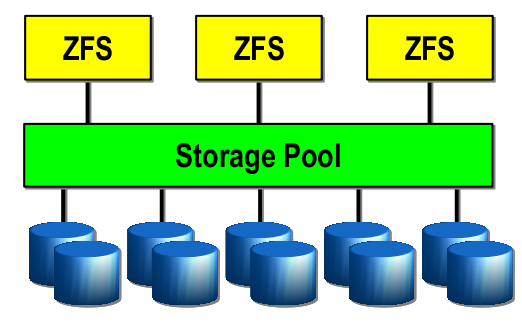
\includegraphics[width=5cm]{figs/pools.png}
%  \caption   Easy: insert a ``volume'' to cobble disks together.
\end{center}
\end{figure}

\end{frame}

\begin{frame}
  \frametitle{RAID-Z}

  \begin{itemize}
\small
    \item RAID no estándar: específico de ZFS.
    \item Similar a RAID 5, pero evita el \textit{write hole} de RAID 5 (si se produce un apagón durante una escritura, paridad o datos pueden quedar inconsistentes/corruptos).
    \item Existe también RAID-Z2 que dobla (o triplica) la estructura de partidad alcanzando resultados similares a RAID 6. 
    \item En Julio de 2009, se incorporó RAIDZ de triple paridad a OpenSolaris. 
    \item No precisa ningún hardware especial.
  \end{itemize}

\normalsize

\begin{figure}[h]
\begin{center}
  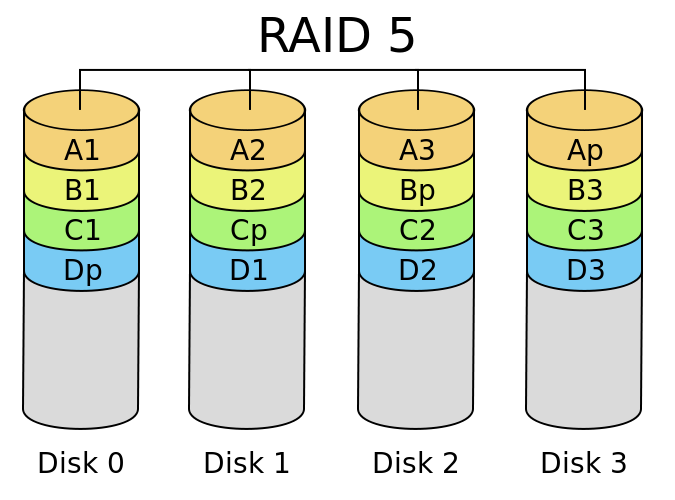
\includegraphics[width=3cm]{figs/RAID_5.png}
%  \caption  RAID level 5.
\end{center}
\end{figure}

\end{frame}


\begin{frame}
  \frametitle{}
  \begin{itemize}
    \item Demo
  \end{itemize}
\end{frame}

%%%%%%%%%%%%%%%%%%%%%%%%%%%%%%%%%%%%%%%%%%%%%%%%%%%%%%%%%%%%%%%%%%%%%%%%%

% Portada final
\frame{
\maketitle
\begin{center}

\includegraphics[width=6cm]{format/gsyc-urjc}
\end{center}
}


%Fin de la presentacion
\end{document}


